\documentclass[11pt,a4paper]{article}
\usepackage{acl2015}
\usepackage{times}
\usepackage{url}
\usepackage{latexsym}
\usepackage{tikz}
\usepackage{pgfplots}
\usepackage{pgfplotstable}
\usetikzlibrary{bayesnet}
\usepackage{caption}
\usepackage{subcaption}
\usepackage{graphicx}
\graphicspath{ {images/} }
\setlength\titlebox{5cm}

% Better references, I think
\newcommand{\secref}[1]{Section~\ref{sec:#1}}
\newcommand{\figref}[1]{Figure~\ref{fig:#1}}
\newcommand{\algref}[1]{Algorithm~\ref{alg:#1}}
\newcommand{\tabref}[1]{Table~\ref{tab:#1}}

\newcommand{\relation}[1]{\textsc{#1}}
\newcommand{\pathtype}{\ensuremath{\pi}}

\title{Incorporating Knowledge Graph Features\\
into Relation Extraction Models}

%\author{Dheeru Dua \\
  %Carnegie Mellon University \\
  %{\tt ddua@andrew.cmu.edu} \\\And
  %Matt Gardner \\
  %Carnegie Mellon University \\
  %{\tt mg1@cs.cmu.edu} \\}

\date{}

\begin{document}
\maketitle
\begin{abstract}

  There has been much recent work on the construction of large knowledge bases,
  such as Freebase, NELL, and DBPedia.  These knowledge bases (KBs) have been
  used to provide training data for relation extraction systems and semantic
  parsers, and as databases backing question answering systems, but there has
  been very little work that makes use of these KBs for lower-level natural
  language processing tasks.  We present a simple technique for incorporating
  features from a KB into any graphical model that contains a pairwise factor
  between KB entities.  We apply this idea to a relation extraction model,
  showing striking improvements over prior relation extraction techniques, both
  those that use distant supervision and those that use KB embeddings.

\end{abstract}

\section{Introduction}

It has long been understood that a large collection of common-sense knowledge
is an essential component of any system that will be able to fully understand
natural language.  The Cyc project~\cite{cyc-1995} is one of the more
well-known projects seeking to collect such common-sense knowledge, and the
recent Winograd schema challenge~\cite{winograd-schema-2012} makes it very
clear how necessary this kind of knowledge is in natural language
understanding.  Because of this necessity, there has recently been a surge of
interest in constructing very large knowledge bases (KBs), such as
Freebase~\cite{freebase-2008-bollacker}, NELL~\cite{nell-2015-aaai}, and
DBPedia~\cite{dbpedia-2012-mendes}, which contain facts about people, things,
and places in the world.  These knowledge bases have found use in providing
training data for relation extraction and semantic parsing
models~\cite{riedel-2010-distant-supervision,krishnamurthy-2012-semantic-parsing},
and forming the foundation of question answering systems such as Google's
search and Apple's Siri.

One place where these knowledge bases have not typically found use is in
lower-level natural language models.  While it is now understood how to parse a
question into an executable query over a structured knowledge base, it is less
clear how to tractably incorporate a knowledge base into a model for parsing or
part-of-speech tagging.  In this work, we take a step in that direction by
presenting a general technique for incorporating features generated from a
knowledge base into \emph{any} graphical model that contains a pairwise factor
between KB entities.

Our method is inspired by the Path Ranking Algorithm~\cite[PRA]{lao-2010-pra},
a method for constructing feature matrices over node pairs in a graph.  Almost
all prior work with PRA has used the constructed feature matrix to perform link
prediction in the graph; when the graph corresponds to a knowledge base, this
is the task of knowledge base completion, and most work with PRA has focused
exclusively on this task~\cite{lao-2011-pra2,lao-2012-syntactic-pra,%
dong-2014-knowledge-vault,gardner-2013-latent-pra,gardner-2014-vector-space-pra}.
However, the feature matrices constructed by PRA need not be used only in a
logistic regression classifier; they can be included as factors in arbitrary
graphical models.

As an initial proof-of-concept of this idea, we add a PRA feature matrix as a
factor in an off-the-shelf distantly-supervised relation extraction model, the
MultiR system of Hoffmann et al.~\shortcite{hoffmann-2011-distant-supervision}.
We chose this model for our initial experiment because the choice of KB is
obvious (as they use a KB to obtain distantly-supervised training examples),
and deciding how to incorporate a PRA factor is not difficult.  In contrast,
finding a suitable KB for a parsing model, as well as adding a factor in a way
that still allows for efficient inference, are much more challenging.  However,
the gains we achieve by adding PRA features into the MultiR model are quite
substantial, and we believe they provide sufficient motivation to solve the
challenges of incorporating these same ideas into more low-level NLP models.

In the remainder of this paper, we first briefly describe the PRA and MultiR
models, as well as other related work, then we describe how we incorporate PRA
features into MultiR.  We then present an experimental comparison between our
PRA-augmented MultiR model with various techniques from prior work, showing
that our method substantially outperforms prior techniques in both aggregate
and sentential relation extraction.

\section{The Path Ranking Algorithm}

The path ranking algorithm was introduced by Lao and Cohen in 2010.  It is a
two-step process for generating a feature matrix over node pairs in a graph.
The first step finds a set of potentially useful path types that connect the
node pairs, which become the columns of the feature matrix.  A \emph{path type}
\pathtype{} is a sequence of edge types in the graph, such as
-\relation{CityInState}-\relation{StateInCountry}- (this particular path type
would be highly predictive of instances of \relation{CityInCountry}).  These
path types are found by performing a search over the graph, looking for path
types that commonly connect the source and target nodes of the training
instances for a particular relation.  Once selected, each path type becomes a
column in the constructed feature matrix (where rows correspond to entity
pairs).

Once a set of path types has been found, the second step of PRA then computes
the values in the feature matrix.  The value for a particular cell in the
matrix is the probability of starting at the source node of an entity pair,
following the path type corresponding to the column of the matrix, and arriving
at the target node of the entity pair: $p(t|s,\pathtype)$.  These probabilities
can be computed with a breadth-first search, with matrix multiplications, or by
using random walks to perform rejection sampling.

After this two-step process has computed a feature matrix, typical uses of PRA
then learn a logistic regression classifier to score new entity pairs and
perform knowledge base completion.  In this work, however, we inject the
feature matrix into a more complex graphical model, the MultiR model for
performing relation extraction, described in the next section.  Additionally,
because the second step of PRA is very computationally expensive, and some
experimentation showed that using binary features performs just as well, we
only use the first step of PRA to compute a binary feature matrix.

\section{MultiR}

The MultiR algorithm~\cite{hoffmann-2011-distant-supervision} is a
probabilistic graphical model for performing relation extraction with distant
supervision.  The model is \emph{distantly supervised} because while it makes
predictions on individual sentences, it has no annotated sentences as training
data.  Instead, it obtains supervision by aligning entity pairs seen in a
knowledge base with entity pairs seen in sentences, and assumes that at least
one of the sentences for a particular entity pair expresses the relationship
seen in the KB.  The model also allows for more than one relationship to exist
between a pair of entities, to account for the fact, e.g., that a person might
be born in a nation, have citizenship there, and be president of that nation,
all of which are typically separate relations in a KB.  The model is shown in
\figref{multir}, where $S$ is the set of sentences between any two entities
$e_1$, $e_2$ $\in$ E and $Z_i$'s are the latent variables that range over all
relation names and a distinct value None. The model outputs a binary relation
vector Y, with indicator bits for each relation.  It is trained using an online
perceptron-style algorithm.

\section{Other Related Work}
\label{sec:related-work}

We briefly mention here a few other pieces of related work, particularly those
that we will compare our work against.  Surdeanu et
al.~\shortcite{surdeanu-2012-relation-extraction} presented MIML-RE, which is
very similar to the MultiR algorithm, but relaxes some of the hard constraints
used by MultiR.  Weston et
al.~\shortcite{weston-2013-connecting-language-and-kb} is the work that is most
similar to ours, in that they also attempted to add information from a
knowledge base to a relation extraction model.  They used neural embeddings,
however, instead of the factor-based approach that we take in this paper, so
their technique is not as widely applicable as ours.

\section{PRA-Augmented MultiR}
\label{sec:pra-augmented-multir}

There are two options for adding a PRA factor into the MultiR model.  The first
(and more natural) place to add the factor is once per entity pair, as an
additional component to the factor connecting the $Y$ and $Z_i$ variables.
This is shown in \figref{per-entity-pair}.  The issue with this placement is
that the factor connecting $Y$ and $Z_i$ is a determinstic OR, and the model is
trained using an at-least-once assumption; this means that if the model can
explain the existence of a relationship between an entity pair with the PRA
factor, it will tend to not learn from the sentences for that entity pair.

An alternate placement is to include the PRA features as an additional
component of every mention of the entity pair, shown in \figref{per-mention}.
One way this can be thought of is as a stronger kind of supervision; the
stronger an entity exhibits a particular relationship, as determined by the PRA
features, the more likely the dependency parse features of the MultiR model are
to be upweighted for that sentence.  When judging aggregate performance, this
also gives the model access to a much richer set of features than just those
expressed in the corpus.

\begin{figure}[t!]
  \centering
  \begin{subfigure}[t]{2.0cm}
    \begin{tikzpicture}
       \node[latent]          (y)   {$Y$};
       \node[latent, below=2cm of y]            (zi) {$Z_i$} ;
       \factor[below=1.2cm of y] {y-f} {} {y} {zi} ;
       \factor[right=0.3cm of zi] {zi-f} {$f_{s}$} {zi} {} ;
        \plate {r} {
          (y)
        } {$R$} ; %
       \plate {s} {
          (zi)(zi-f)
        } {$S$} ; %
      \plate {ee} {
          (r)(s)
        } {$EXE$} ; %
    \end{tikzpicture}
    \caption{MultiR}
    \label{fig:multir}
  \end{subfigure}
  ~
  \begin{subfigure}[t]{2.0cm}
    \begin{tikzpicture}
       \node[latent]          (y)   {$Y$};
       \node[latent, below=2cm of y]            (zi) {$Z_i$} ;
       \factor[below=1.2cm of y] {y-f} {} {y} {zi} ;
       \factor[right=0.3cm of zi] {zi-f} {$f_{s}$} {zi} {} ;
       \factor[right=of y-f] {zi-fpra} {$f_{pra}$} {y-f} {} ;
        \plate {r} {
          (y)
        } {$R$} ; %
       \plate {s} {
          (zi)(zi-f)
        } {$S$} ; %
      \plate {ee} {
          (r)(s)
        } {$EXE$} ; %
    \end{tikzpicture}
    \caption{Per Entity-pair}
    \label{fig:per-entity-pair}
  \end{subfigure}
  ~
  \begin{subfigure}[t]{2.0cm}
    \begin{tikzpicture}
       \node[latent]          (y)   {$Y$};
       \node[latent, below=2cm of y]            (zi) {$Z_i$} ;
       \factor[below=1.2cm of y] {y-f} {} {y} {zi} ;
       \factor[right=0.3cm of zi] {zi-f} {$f_{s}$} {zi} {} ;
       \factor[left=0.3cm of zi] {zi-fpra} {$f_{pra}$} {zi} {} ;
        \plate {r} {
          (y)
        } {$R$} ; %
       \plate {s} {
          (zi)(zi-f)(zi-fpra)
        } {$S$} ; %
      \plate {ee} {
          (r)(s)
        } {$EXE$} ; %
    \end{tikzpicture}
    \caption{Per Mention}
    \label{fig:per-mention}
  \end{subfigure}
  \caption{Plate notation of the model}
\end{figure}


\section{Experiments}

To evaluate the performance of this model, we use the dataset developed by
Riedel et al.~\shortcite{riedel-2010-distant-supervision}, which aligns
Freebase relations with a New York Times corpus.  The dataset contains a number
of sentence mentions for each entity pair. The entities are extracted from
sentences by Stanford Named Entity Tagger~\cite{finkel-2005-non-local-ie},
spanning across 52 freebase relations.  The sentence level features include the
part of speech tags, named entities and dependency tree paths.  Many systems
have evaluated their performance on this dataset, including MultiR and the two
systems mentioned in \secref{related-work}, MIML-RE and Weston's embedding
method, allowing us to easily compare performance with those methods.  The
evaluation protocol sorts all predictions for all relations by confidence and
computes a precision-recall curve over those predictions.  We evaluate
extraction performance in aggregate (comparing predicted $Y$ values to truth
from the KB), and at the sentence level (comparing predicted $Z_i$ values to
human-annotated $Z_i$ values in the test set).

To extract PRA features, we used somewhat outdated dump of the Freebase graph,
excluding some of the largest relations (including those that are not really
relevant to the relations in the dataset we used, such as relations under
\relation{/user} and \relation{/common}, and relations dealing with things like
individual music tracks and TV episodes).  We removed any direct edges between
entity pairs in the training and test data, then ran the first step of PRA to
produce a binary feature matrix.  We then added this matrix as a factor to the
MultiR model as described in \secref{pra-augmented-multir}.  We found that
because this new factor increased the size of the feature space, additional
regularization was needed.  We added an L2 regularization parameter to the
model, which we tuned using 5-fold cross validation on the training data.  This
significantly improved the performance of our augmented model, though a similar
addition to MultiR did not improve performance, so we did not include it in our
final experiments.

We first present a comparison of aggregate extraction performance between the
ways of augmenting MultiR with PRA features.  \figref{our-comparison} shows the
results of the two different augmentations, along with a baseline of using just
the PRA feature as a single entity pair mention, so we can get some sense of
how much of the gain from our methods comes from the PRA features themselves,
and not from interactions between PRA and dependency path features.

\begin{figure}
  \centering
  \begin{tikzpicture}
    \begin{axis}[xlabel=Recall, ylabel=Precision, no markers,width=\columnwidth]
      \addplot table [y=Precision, x=Recall]{data/pra_per_mention.tsv};
      \addlegendentry{PRA Per Mention}
      \addplot table [y=Precision, x=Recall]{data/pra_per_entity.tsv};
      \addlegendentry{PRA Per Entity}
      \addplot [mark=none, green] table [y=Precision, x=Recall]{data/pra_only.tsv};
      \addlegendentry{PRA Only}
    \end{axis}
  \end{tikzpicture}
  \caption{Aggregate extraction performance of the augmented MultiR methods
  introduced in this paper.}
  \label{fig:our-comparison}
\end{figure}

Next, \figref{prior-work-comparison} shows a comparison between our best
augmented model and prior work on aggregate extraction performance.  As can be
seen from the figure, our method substantially outperforms all prior work,
including models that just used dependency path features (MultiR and MIML-RE)
and models that combined KB embeddings with dependency path features (WESTON).

\begin{figure}
  \centering
  \begin{tikzpicture}
    \begin{axis}[xlabel=Recall, ylabel=Precision, no markers,width=\columnwidth]
      \addplot table [y=Precision, x=Recall]{data/hoffmann.tsv};
      \addlegendentry{Hoffmann}
      \addplot table [y=Precision, x=Recall]{data/weston.tsv};
      \addlegendentry{Weston}
      \addplot table [y=Precision, x=Recall]{data/pra_per_mention.tsv};
      \addlegendentry{Ours}
    \end{axis}
  \end{tikzpicture}
  \caption{Aggregate extraction performance of our method compared with several
  methods from prior work.}
  \label{fig:prior-work-comparison}
\end{figure}

Lastly, we present a comparison of sentential extraction performance between
MultiR and our augmented version.  Because PRA features might mislead the model
to predict a relation instance that is not actually expressed in a particular
sentence, we also experimented with only using the PRA features at training
time, removing them during testing.  \figref{sentential-comparison} shows the
results of this comparison.  PRA-augmented MultiR performs slightly better here
than MultiR, and, somewhat surprisingly, using PRA features only at training
time performs substantially better still.  We believe this is because the
presence of the PRA features at training time gives the model a stronger and
better supervision signal, resulting in better learned weights for the
dependency features.

\begin{figure}
  \centering
  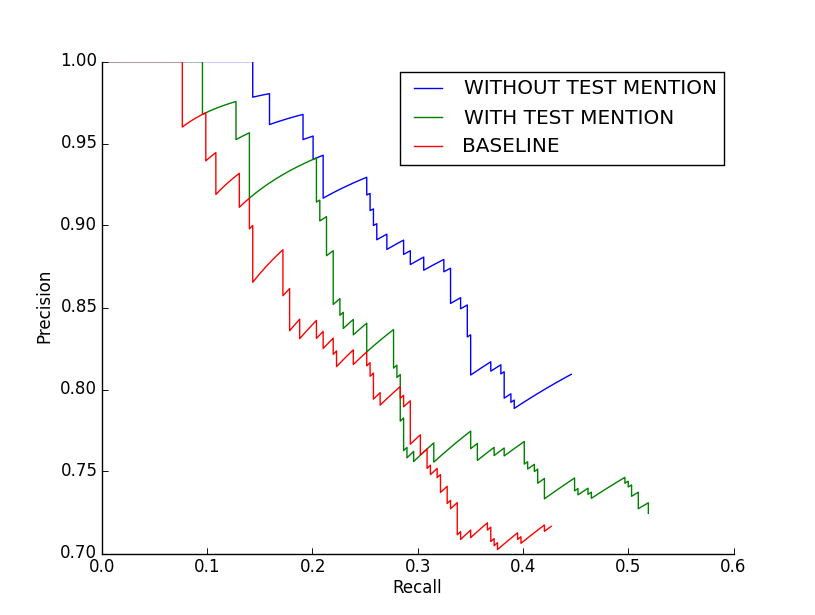
\includegraphics[width=8cm,height=6cm]{senPR.png}
  \caption{Sentential extraction performance of our method compared with
  MultiR.}
  \label{fig:sentential-comparison}
\end{figure}

\section{Conclusion}

We have addressed the problem of incorporating features from a knowledge base
into low-level natural language processing models.  We introduced a simple
technique that computes a PRA feature matrix from a knowledge base and
incorporates it as a factor in arbitrary graphical models.  As an initial
proof-of-concept of this general technique, we showed dramatic improvements
when using this idea to augment an off-the-shelf relation extraction model,
MultiR.  We believe this result amply shows the utility of this technique, and
hope to similarly apply it to other low-level NLP models in the future.

\bibliographystyle{acl}
\bibliography{bib}

\end{document}
